\documentclass[portuguese]{sbc2025}

\usepackage[misc,geometry]{ifsym}
\usepackage{aas_macros}
\usepackage[bottom]{footmisc}
\usepackage{tabularray}
\usepackage{afterpage}
\usepackage{url}
\usepackage{pifont}

\setcitestyle{square}

\definecolor{engtitle}{rgb}{0.5,0.5,0.5}
\definecolor{orcidlogo}{rgb}{0.37,0.48,0.13}
\definecolor{unilogo}{rgb}{0.16, 0.26, 0.58}
\definecolor{maillogo}{rgb}{0.58, 0.16, 0.26}
\definecolor{darkblue}{rgb}{0.0,0.0,0.0}
\hypersetup{colorlinks,breaklinks,
            linkcolor=darkblue,urlcolor=darkblue,
            anchorcolor=darkblue,citecolor=darkblue}

\jid{REIC}
\jtitle{Revista Eletrônica de Iniciação Científica em Computação, 2026}
\issn{3085-8461}
\copyrightstatement{This work is licensed under a Creative Commons Attribution 4.0 International License}
\jyear{2026}

\category{Artigo de Pesquisa/Research Paper}
\title{Chopper Tracker: Protótipo de Sequenciador no Paradigma Tracker com Integração em DAWs para Produção Musical}
\engtitle{\textcolor{engtitle}{Chopper Tracker: A Tracker-Paradigm Sequencer Prototype with DAW Integration for Music Production}}

\author[Ribeiro 2026]{
\affil{\textbf{Yan Ribeiro}~\textcolor{blue}{\faEnvelopeO}~~[{Centro Federal de Educação Tecnológica Celso Suckow da Fonseca (CEFET/RJ)}~|\href{mailto:yanribeironasc@gmail.com}{~{\textit{yanribeironasc@gmail.com}}}~]}
}

\begin{document}

\begin{frontmatter}

\maketitle

\begin{mail}
Centro Federal de Educação Tecnológica Celso Suckow da Fonseca (CEFET/RJ), Unidade Maria da Graça, Rua Miguel Ângelo, 96, Maria da Graça, Rio de Janeiro, RJ, 20785-223, Brasil.
\end{mail}

\begin{abstract-pt}
Este trabalho apresenta o Chopper Tracker, um protótipo de sequenciador no paradigma tracker voltado ao fluxo de trabalho de chopping de samples e à integração em Digital Audio Workstations (DAWs). O paradigma tracker oferece controle passo a passo sobre cada hit percussivo, sendo amplamente adotado em gêneros como drum \& bass e breakcore. Contudo, trackers modernos como OpenMPT e Renoise são aplicações autônomas de desktop: utilizá-los exige que o produtor abandone seu ambiente de DAW, fragmentando o fluxo criativo. Dentro das próprias DAWs, por outro lado, não existe nenhum plugin que ofereça o paradigma tracker integrado ao fluxo de chopping. O Chopper Tracker foi desenvolvido para demonstrar a viabilidade desse conceito, reunindo em um único ambiente um editor de áudio com fatiamento automático por detecção de transientes, um sequenciador tracker, um analisador harmônico, um piano roll e um sintetizador. A implementação atual funciona como aplicação web, exportando WAV e MIDI para uso imediato em DAWs, e serve de base para a evolução natural do projeto: um plugin nos formatos VST/CLAP.
\end{abstract-pt}

\begin{abstract-en}
This paper presents Chopper Tracker, a tracker-paradigm sequencer prototype designed for the sample chopping workflow and DAW integration. The tracker paradigm provides step-by-step control over individual percussive hits and is widely adopted in genres such as drum \& bass and breakcore. However, modern trackers such as OpenMPT and Renoise are standalone desktop applications: using them requires producers to leave their DAW environment, fragmenting the creative workflow. Within DAWs themselves, no plugin currently offers the tracker paradigm integrated with a chopping workflow. Chopper Tracker was developed to demonstrate the viability of this concept, combining in a single environment an audio editor with automatic transient-based slicing, a tracker sequencer, a harmonic analyzer, a piano roll, and a synthesizer. The current implementation runs as a web application that exports WAV and MIDI for immediate use in DAWs, and serves as the foundation for the project's natural evolution: a VST/CLAP plugin.
\end{abstract-en}

\begin{pchaves}
Produção Musical, Sample Chopping, Plugin VST, Tracker, Sequenciamento de Áudio, DAW.
\end{pchaves}

\begin{keywords}
Music Production, Sample Chopping, VST Plugin, Tracker, Audio Sequencing, DAW.
\end{keywords}

\end{frontmatter}


\section{Introdução}

A produção musical digital se consolidou em torno das Digital Audio Workstations (DAWs), que centralizaram em um único ambiente as etapas de gravação, edição, arranjo e mixagem de áudio \citep{izhaki2012mixing}. No ecossistema atual, DAWs como FL Studio, Ableton Live e Bitwig Studio dominam o mercado de produção eletrônica. Em paralelo, existe uma categoria distinta de software musical, o tracker, organizado como uma grade onde cada coluna representa um instrumento e cada linha representa um passo no tempo \citep{roads1996computer}. Ao digitar notas célula a célula, o produtor tem controle preciso sobre cada hit percussivo individual, tornando o paradigma tracker a escolha consagrada para gêneros como drum \& bass, jungle e breakcore, onde o microgerenciamento de cada fragmento rítmico é central para a composição.

O Renoise é o principal representante moderno desse paradigma: um tracker completo, com suporte a plugins VST, que permite ao produtor fazer chopping de samples com um nível de detalhe por passo que nenhuma DAW convencional oferece nativamente \citep{renoise}. O problema é que Renoise e FL Studio são concorrentes: são ambientes de produção autônomos, e o produtor precisa escolher um ou outro. Quem produz no FL Studio abre mão do microgerenciamento do Renoise; quem produz no Renoise abre mão do ecossistema, dos plugins e do fluxo de arranjo do FL Studio.

Dentro do FL Studio, a ferramenta mais próxima do fluxo de chopping é o Slice~X, que permite importar um sample, fatiar por transientes e mapear os slices a notas MIDI. O Slice~X resolve a integração com o ambiente de produção, mas seu paradigma de interface, baseado em pad e piano roll, não oferece o mesmo nível de microgerenciamento que o Renoise proporciona célula a célula. A mesma limitação se aplica ao Simpler no Ableton Live e ferramentas equivalentes em outras DAWs. A lacuna é precisa: não existe um plugin que leve o paradigma de microgerenciamento do Renoise para dentro do FL Studio.

Este trabalho apresenta o Chopper Tracker, um protótipo que demonstra a viabilidade de preencher essa lacuna. A proposta é um sequenciador no paradigma tracker que funciona como plugin dentro de uma DAW, reunindo o nível de controle passo a passo do Renoise com a integração nativa ao ambiente de produção do FL Studio. A implementação atual opera como uma aplicação web, exportando WAV e MIDI para integração imediata com qualquer DAW, e serve de prova de conceito para a evolução natural do projeto: um plugin nos formatos VST/CLAP. O sistema integra um editor de áudio com fatiamento automático por detecção de transientes, um sequenciador no paradigma tracker, um analisador harmônico, um piano roll e um sintetizador.

\begin{figure}[h!]
\begin{center}
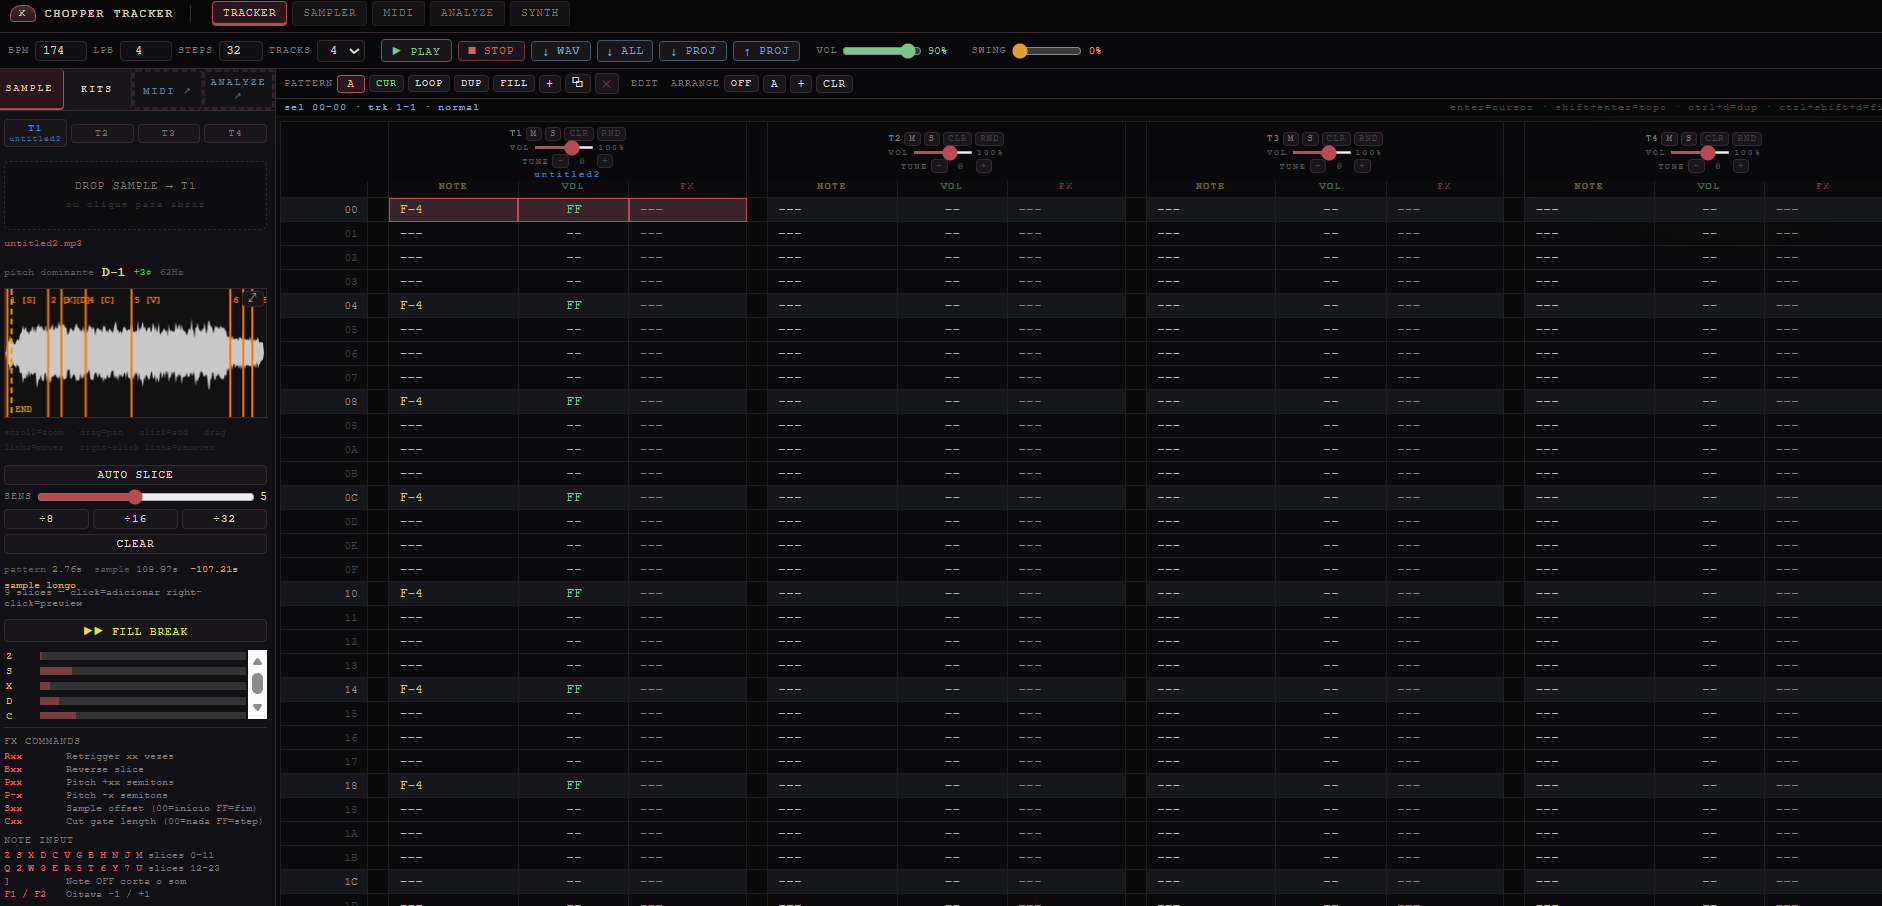
\includegraphics[width=\columnwidth]{sequenciador.png}
\caption{Interface do Sequenciador do Chopper Tracker.}\label{fig:sequenciador}
\end{center}
\end{figure}

\section{Fundamentação Teórica}

\subsection{Samples e Música Baseada em Amostras}

O termo sample designa qualquer trecho de áudio extraído de uma gravação preexistente e reutilizado em uma nova composição \citep{schloss2004making}. A prática do reaproveitamento sonoro tem raízes na música concreta dos anos 1940, com Pierre Schaeffer, e se consolidou como forma de expressão autônoma no hip-hop norte-americano da década de 1980, impulsionada por equipamentos como o Akai MPC60. No presente, o sampling é reconhecido como técnica legítima de composição e é protegido juridicamente em muitos países sob o conceito de \textit{transformative use}, sendo culturalmente celebrado como forma de homenagem e recontextualização.

\subsection{Breaks e a Técnica de Chopping}

Um break é o trecho específico de uma gravação em que apenas a percussão toca, sem vocais ou melodia. O termo deriva da prática de DJs do Bronx, Nova York, nos anos 1970, que estendiam esse momento de uma faixa para que o público pudesse dançar, manipulando dois discos de vinil idênticos em toca-discos separados \citep{chang2005cant}. Quando isolado e sampleado, esse trecho se torna a base rítmica de uma nova faixa.

A técnica de chopping consiste em fatiar esse break em fragmentos menores, denominados slices, e reorganizá-los em padrões rítmicos originais. Cada slice corresponde a um ataque percussivo individual, como bumbo, caixa ou chimbal, e pode ser atribuído a uma nota em um sequenciador. O resultado são grooves com variações de timing e velocidade que transcendem as limitações físicas de qualquer baterista humano. O chopping é a linguagem composicional central do drum \& bass, jungle e breakcore \citep{schloss2004making}.

\subsection{Trackers como Paradigma de Sequenciamento}

Um tracker é um software musical cujo paradigma de entrada se baseia em uma tabela: cada coluna representa um instrumento independente e cada linha representa um passo no tempo. O músico digita notas diretamente pelo teclado do computador, célula a célula, e o programa executa a grade de cima para baixo em loop, como uma partitura \citep{roads1996computer}. O paradigma nasceu em 1987 com o Ultimate Soundtracker, desenvolvido por Karsten Obarski para o Amiga, e permanece como interface preferida em gêneros como drum \& bass e breakcore, onde o controle preciso sobre cada hit de bateria é essencial.

\subsection{Digital Audio Workstations}

Uma Digital Audio Workstation (DAW) é um sistema de software que centraliza as etapas de gravação, edição, arranjo, mixagem e masterização de áudio \citep{izhaki2012mixing}. Exemplos amplamente utilizados incluem Ableton Live, FL Studio e Bitwig Studio. Embora DAWs modernas ofereçam recursos de fatiamento de áudio integrados, como o Simpler e o Sampler do Ableton Live, esses recursos são componentes de ambientes de propósito geral e não proveem um fluxo de trabalho especializado para o chopping de breaks.

\subsection{Web Audio API}

A Web Audio API é uma especificação do W3C que define uma interface de alto nível para processamento e síntese de áudio no navegador \citep{webaudioapi2021}. Seu modelo é baseado em um grafo de nós de processamento de áudio (\textit{AudioNode}s) conectados a um contexto de destino (\textit{AudioContext}). A especificação provê nós para reprodução de buffers (\textit{AudioBufferSourceNode}), controle de ganho (\textit{GainNode}), análise espectral (\textit{AnalyserNode}) e renderização offline (\textit{OfflineAudioContext}), esta última essencial para a exportação de áudio sem dependência de processamento em tempo real.


\section{Trabalhos Relacionados}

A análise das ferramentas existentes evidencia dois grupos que resolvem metade do problema cada um, deixando clara a lacuna que o Chopper Tracker busca preencher.

\subsection{Renoise e o Paradigma Tracker}

O Renoise \citep{renoise} é o tracker moderno mais completo disponível: suporta plugins VST/VSTI, MIDI, fatiamento automático de samples e oferece um ambiente de produção inteiro dentro do paradigma tracker. Para produtores de drum \& bass e breakcore, o Renoise é referência de microgerenciamento rítmico: cada hit percussivo ocupa uma célula própria na grade, podendo receber configurações individuais de volume, pitch, efeitos e retrigger, algo que nenhum sampler convencional replica com o mesmo nível de granularidade.

O OpenMPT \citep{openmpt}, tracker de código aberto focado na preservação de formatos históricos como .MOD e .XM, reforça que esse paradigma tem comunidade ativa e casos de uso consolidados. O problema de ambos não está no paradigma; está na arquitetura como aplicações autônomas. Renoise e FL Studio são concorrentes diretos: são ambientes de produção completos, e o produtor escolhe um ou outro. Quem quer o microgerenciamento do Renoise abre mão do ecossistema do FL Studio, e vice-versa.

\subsection{Slice X e Ferramentas de Chopping em DAWs}

Dentro do FL Studio, o Slice~X é a ferramenta nativa de chopping: importa um sample, detecta transientes e mapeia os slices a notas MIDI, funcionando como um instrumento dentro do ambiente de produção. O Simpler e o Sampler do Ableton Live cumprem papel equivalente em sua DAW. A integração com o restante do projeto, mixer, plugins, arranjo, é o ponto forte dessas ferramentas.

A limitação está no paradigma de interface. O Slice~X opera com piano roll e mapeamento por pad: o produtor programa os hits em uma grade MIDI genérica, sem a visibilidade célula a célula que o tracker oferece. No Renoise, cada passo da grade é uma unidade compositiva com parâmetros próprios; no Slice~X, o mesmo hit é um evento MIDI numa faixa genérica. Para o fluxo de chopping de um break, essa diferença de granularidade é significativa.

\subsection{A Lacuna}

O cenário coloca o produtor diante de uma escolha binária: o microgerenciamento do Renoise ou a integração do FL Studio. Não existe plugin que traga o paradigma tracker para dentro de uma DAW. O Chopper Tracker é a proposta de preencher exatamente esse espaço: um sequenciador com o nível de controle do Renoise funcionando como plugin dentro do FL Studio ou de qualquer outra DAW compatível com VST/CLAP.


\section{Desenvolvimento da Ferramenta}

Este capítulo apresenta a arquitetura da solução, as tecnologias utilizadas, a descrição de cada módulo, o pipeline de trabalho proposto e os algoritmos centrais que sustentam o funcionamento do Chopper Tracker. A implementação foi conduzida como prova de conceito na plataforma web, ambiente que permite iteração rápida sobre a interface e os algoritmos sem as restrições do modelo host/plugin. As decisões de arquitetura foram tomadas com a portabilidade para plugin em mente: estado centralizado, processamento de áudio desacoplado da interface e saídas em formatos padrão da indústria (WAV e MIDI).

\subsection{Arquitetura da Solução}

A arquitetura do Chopper Tracker é baseada em uma aplicação web cliente que executa inteiramente no navegador, sem dependência de servidor remoto. O estado global da aplicação é centralizado no módulo \texttt{js/state.js}, que mantém o buffer de áudio carregado, os slices detectados, o padrão do sequenciador, o BPM e as configurações de canais. A comunicação entre os módulos se dá por importação direta de módulos ES6, sem camada de mensagens ou barramento de eventos externo.

A aplicação é composta por cinco páginas HTML independentes, cada uma correspondendo a um módulo, vinculadas por uma barra de navegação persistente: \texttt{index.html} (Sequenciador), \texttt{sampler.html} (Editor de Áudio), \texttt{analyze.html} (Analisador), \texttt{midi.html} (Piano Roll) e \texttt{synth.html} (Sintetizador). A inicialização é realizada por um servidor HTTP simples em Python (\texttt{server.py}), que serve os arquivos estáticos, contornando as restrições de CORS que o navegador impõe ao carregamento de módulos ES6 a partir do sistema de arquivos local. Scripts de lote (\texttt{.bat}) automatizam a execução no ambiente Windows.

\begin{figure}[h!]
\begin{center}
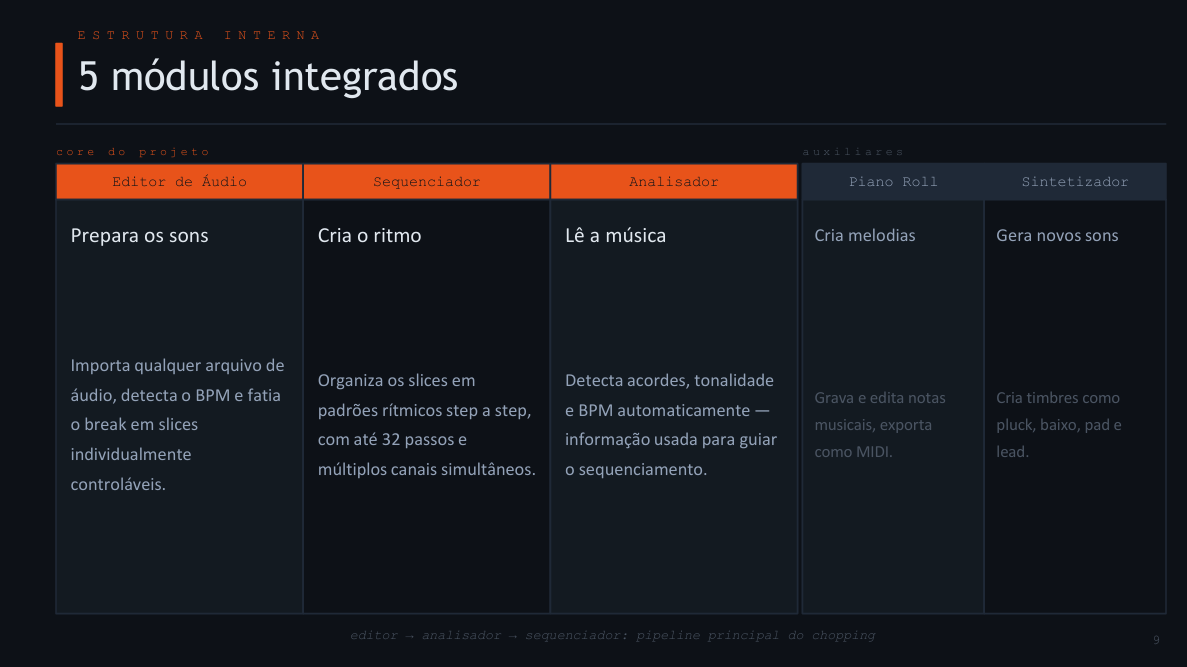
\includegraphics[width=\columnwidth]{arquitetura.png}
\caption{Diagrama de arquitetura modular do Chopper Tracker.}\label{fig:arquitetura}
\end{center}
\end{figure}

\subsection{Tecnologias Utilizadas}

\subsubsection{JavaScript (ES6 Modules)}

A aplicação foi desenvolvida inteiramente em JavaScript nativo, sem frameworks ou bibliotecas de terceiros. A modularização utiliza o sistema de módulos ES6 (\texttt{import}/\texttt{export}), com cada responsabilidade encapsulada em um arquivo separado dentro do diretório \texttt{js/}: \texttt{audio.js}, \texttt{exporter.js}, \texttt{kits.js}, \texttt{main.js}, \texttt{sequencer.js}, \texttt{slicer.js}, \texttt{state.js}, \texttt{tracker-ui.js} e \texttt{waveform-ui.js}.

\subsubsection{Web Audio API}

A Web Audio API \citep{webaudioapi2021} é a fundação de todas as operações de áudio da aplicação. O módulo \texttt{js/audio.js} gerencia o \texttt{AudioContext} global e a reprodução de slices individuais com controle de volume e pitch via \texttt{AudioBufferSourceNode}. O agendamento preciso de eventos sonoros para o sequenciador é realizado pelo mesmo módulo. A exportação WAV utiliza o \texttt{OfflineAudioContext} para renderizar o padrão completo em tempo não real.

\subsubsection{HTML5 Canvas e CSS}

A interface é construída com HTML5 e CSS nativo. O módulo \texttt{js/waveform-ui.js} utiliza o elemento \texttt{<canvas>} para renderizar a forma de onda do áudio carregado e os marcadores de slice. O módulo \texttt{js/tracker-ui.js} constrói dinamicamente a grade do sequenciador via manipulação do DOM, criando células editáveis para cada combinação de passo e canal.

\subsubsection{Python (Servidor HTTP Local)}

Um servidor HTTP simples em Python (\texttt{server.py}) serve os arquivos estáticos da aplicação. Sua função é exclusivamente contornar a política de mesma origem (\textit{same-origin policy}) do navegador, que bloqueia a importação de módulos ES6 a partir de URLs \texttt{file://}. Não há lógica de negócio no servidor: todo o processamento de áudio ocorre no cliente.

\subsection{Módulos da Plataforma}

\subsubsection{Editor de Áudio}

O Editor de Áudio é o módulo de entrada do pipeline de chopping. Ele permite importar qualquer arquivo de áudio nos formatos WAV, MP3 ou FLAC, ou colar diretamente uma URL do YouTube para extração do áudio. Após o carregamento, o módulo exibe a forma de onda completa em um canvas interativo, permitindo seleção visual precisa do trecho desejado. O BPM é detectado automaticamente e a grade de tempo é sincronizada ao andamento do material importado. O usuário pode acionar o fatiamento automático (\textit{Auto Slice}), que aplica o algoritmo de detecção de transientes descrito na Seção~\ref{sec:transientes}, ou inserir pontos de corte manualmente sobre a forma de onda. Cada slice pode ser pré-visualizado individualmente antes de ser enviado ao Sequenciador.

\begin{figure}[h!]
\begin{center}
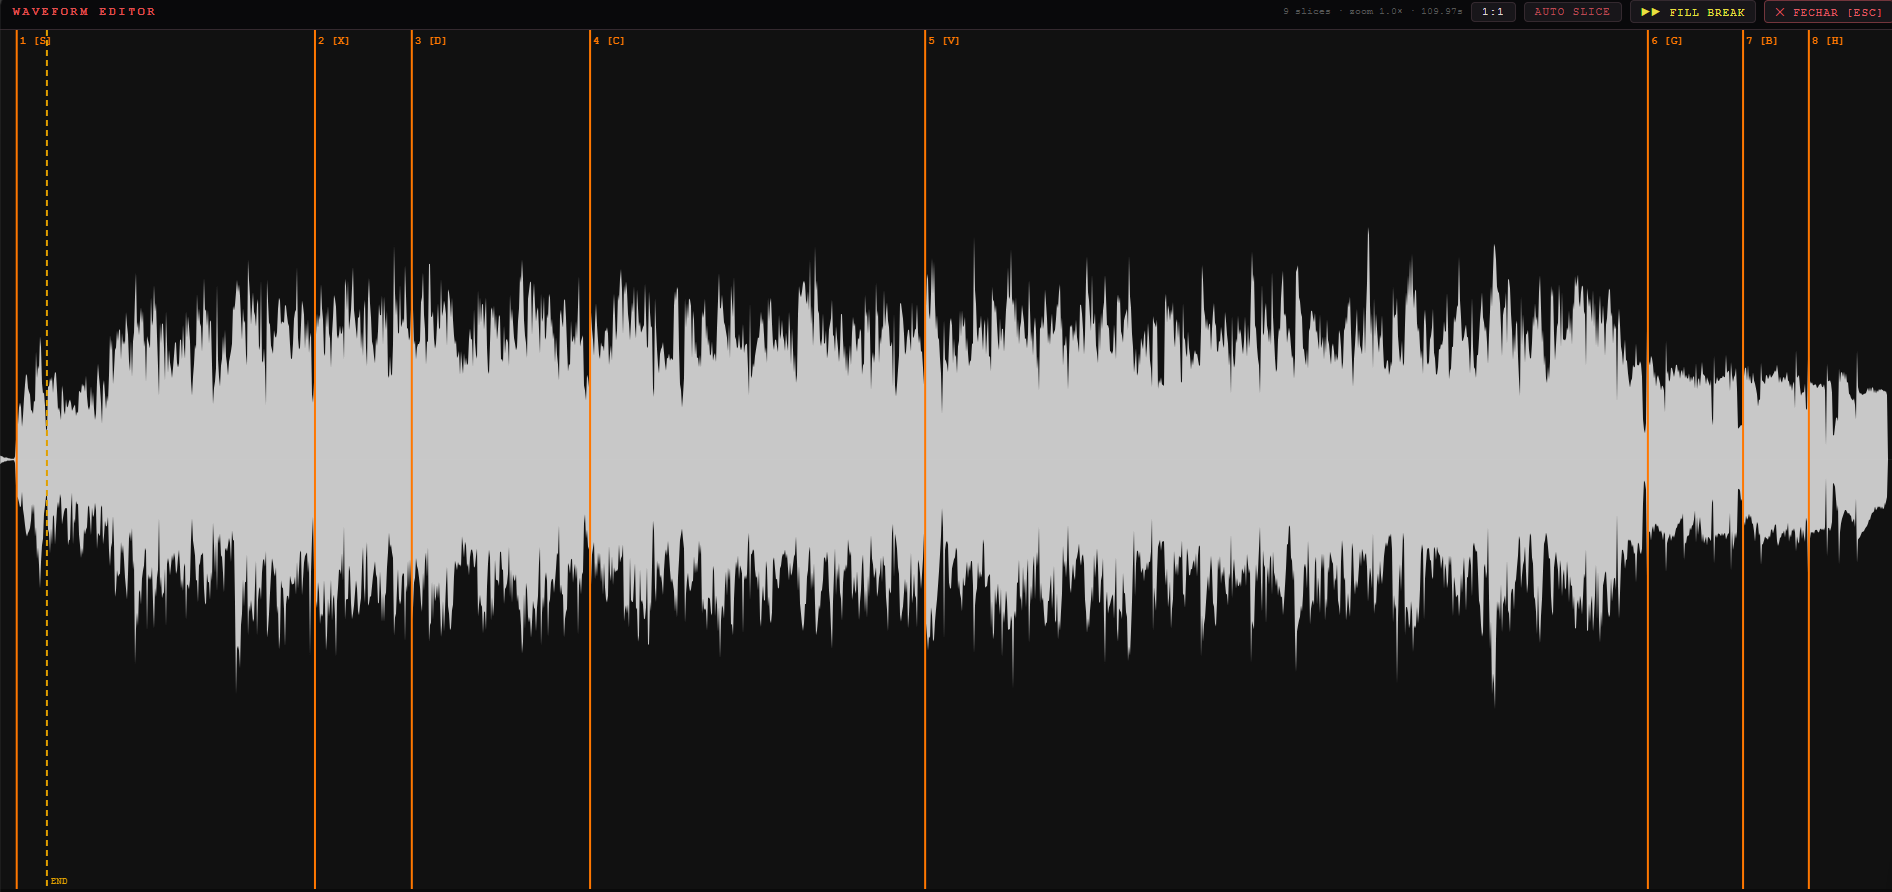
\includegraphics[width=\columnwidth]{editor-audio.png}
\caption{Editor de Áudio com forma de onda e slices detectados automaticamente.}\label{fig:editor}
\end{center}
\end{figure}

\subsubsection{Sequenciador}

O Sequenciador é o módulo central do Chopper Tracker e adota o paradigma tracker de sequenciamento. A interface é organizada como uma grade onde cada coluna representa um canal de instrumento independente e cada linha representa um passo no tempo. O usuário digita notas diretamente pelo teclado do computador, célula a célula, e a grade executa de cima para baixo em loop contínuo. O módulo suporta até 32 passos por padrão e múltiplos canais simultâneos. Cada nota no sequenciador é mapeada a um índice de slice via a função \texttt{sliceIndexToNote}, centralizada em \texttt{js/state.js}. São suportados efeitos por célula: desvio de pitch (\texttt{P}), reprodução reversa (\texttt{B}) e retrigger (\texttt{R}).

\subsubsection{Analisador}

O módulo Analisador realiza análise harmônica e rítmica do áudio carregado de forma automática. São detectados os acordes presentes em cada momento da faixa, a tonalidade global (por exemplo, Dó maior), o BPM e desvios de afinação em cents para correção de pitch. As informações de tonalidade e escala detectadas servem como referência para o sequenciamento no Piano Roll, guiando o produtor na escolha de notas melodicamente coerentes com o sample importado.

\subsubsection{Piano Roll}

O Piano Roll é um módulo auxiliar que permite a criação e edição de sequências de notas MIDI. O usuário pode gravar notas em tempo real ou editá-las diretamente na grade do piano roll. O módulo exporta as sequências no formato MIDI padrão, mapeadas às notas corretas, prontas para importação em qualquer sampler ou instrumento virtual dentro de uma DAW.

\subsubsection{Sintetizador}

O Sintetizador é um módulo auxiliar de geração sonora que permite criar timbres novos dentro da plataforma, sem depender de samples externos. São disponibilizados os arquétipos de síntese mais comuns na produção de drum \& bass: pluck, baixo, pad e lead. Os sons gerados podem ser usados diretamente no Sequenciador como canais adicionais.

\subsection{Pipeline de Trabalho}

O fluxo de trabalho proposto pelo Chopper Tracker organiza a produção em quatro etapas sequenciais, cobrindo do áudio bruto ao arquivo pronto para uso em DAW:

\begin{enumerate}
\item \textbf{Importar:} O produtor arrasta qualquer arquivo de áudio (.wav, .mp3, .flac) para o Editor de Áudio ou cola uma URL do YouTube. O BPM é detectado automaticamente e a grade de tempo é sincronizada ao material importado.

\item \textbf{Recortar:} O produtor seleciona o trecho de percussão desejado e aciona o \textit{Auto Slice}. O algoritmo de detecção de transientes fatia o break em slices individuais, cada um correspondendo a um hit de bateria. A sensibilidade da detecção é ajustável para acomodar beats mais densos ou esparsos.

\item \textbf{Sequenciar:} Os slices são organizados no Sequenciador, cada um atribuído a um canal e a passos da grade, e o padrão rítmico é construído passo a passo. O Analisador pode ser consultado em paralelo para guiar a composição melodicamente.

\item \textbf{Exportar:} O padrão finalizado é exportado como WAV ou MIDI e importado diretamente na DAW de preferência do produtor. O arquivo MIDI já vem mapeado às notas corretas, pronto para uso em qualquer sampler ou instrumento virtual.
\end{enumerate}

\subsection{Algoritmos de Processamento de Áudio}

\subsubsection{Detecção de Transientes}
\label{sec:transientes}

O algoritmo de detecção de transientes, implementado em \texttt{js/slicer.js}, é baseado no monitoramento contínuo do RMS (\textit{Root Mean Square}) do sinal de áudio \citep{bello2005tutorial}. O buffer de áudio é percorrido em janelas de aproximadamente 10~ms, calculadas como $\max(64,\lfloor f_s \cdot 0{,}010 \rfloor)$ amostras, onde $f_s$ é a taxa de amostragem. Para cada janela, o RMS é calculado e comparado ao RMS da janela anterior. Um transiente é detectado quando a razão $\text{rms}/\text{rms}_{\text{prev}}$ excede um limiar configurável, dado por:

$$\text{threshold} = 1 + (10 - s) \cdot 0{,}4$$

onde $s \in [1,10]$ é a sensibilidade definida pelo usuário. Um intervalo mínimo de 30~ms entre transientes consecutivos é imposto para evitar detecções redundantes em sinais com ruído de cauda. O resultado é uma lista de posições de frame que define os pontos de corte dos slices, incluindo o frame zero.

\subsubsection{Agendamento Preciso de Áudio}

O agendamento da reprodução dos slices no Sequenciador é realizado pela Web Audio API com precisão de amostra \citep{webaudioapi2021}. Para cada passo da grade, o módulo \texttt{js/audio.js} calcula o instante absoluto de reprodução no \texttt{AudioContext} com base no BPM e no número de linhas por beat (\texttt{lpb}), e agenda um \texttt{AudioBufferSourceNode} com \texttt{src.start(audioTime)}. Efeitos por célula são aplicados no momento do agendamento: o desvio de pitch é implementado via $\texttt{playbackRate} = 2^{p/12}$, onde $p$ é o número de semitons, e a reprodução reversa é obtida copiando o buffer do slice em ordem invertida para um novo \texttt{AudioBuffer} antes do agendamento.

\subsubsection{Exportação WAV via Renderização Offline}

A exportação do padrão como arquivo WAV é realizada pelo módulo \texttt{js/exporter.js} utilizando o \texttt{OfflineAudioContext} \citep{webaudioapi2021}. Um contexto offline com duração igual ao padrão completo mais dois segundos de cauda é instanciado. Todos os eventos de áudio são agendados nele com a mesma lógica do sequenciador ao vivo. O contexto é então renderizado pelo método \texttt{startRendering()}, produzindo um \texttt{AudioBuffer} final que é codificado como arquivo WAV e disponibilizado ao usuário via \texttt{URL.createObjectURL}, sem qualquer processamento no servidor.


\section{Conclusão}

Este trabalho apresentou o Chopper Tracker, um protótipo que demonstra a viabilidade de um sequenciador no paradigma tracker integrado ao fluxo de trabalho de DAWs. A lacuna identificada é precisa: trackers modernos como OpenMPT e Renoise provam o valor do paradigma, mas existem como aplicações autônomas que exigem que o produtor abandone seu ambiente de produção; os samplers nativos das DAWs resolvem a integração mas abandonam o paradigma. Nenhuma ferramenta existente oferece os dois simultaneamente.

O Chopper Tracker demonstra que essa combinação é realizável. A implementação reúne, em um único ambiente, um editor de áudio com detecção automática de transientes por variação de RMS, um sequenciador no paradigma tracker com até 32 passos e efeitos por célula, um analisador harmônico, um piano roll com exportação MIDI e um sintetizador. O pipeline completo do áudio bruto ao arquivo pronto para DAW foi validado, e os algoritmos centrais, incluindo o agendamento preciso via Web Audio API e a renderização offline para exportação WAV, foram implementados e testados.

A contribuição principal não está na implementação web em si, mas na prova de conceito do modelo: um sequenciador tracker que coexiste com a DAW, em vez de substituí-la. A implementação web foi o veículo de validação; o destino é o plugin. A evolução natural do projeto é o desenvolvimento de uma versão nos formatos VST/CLAP, que embuta o sequenciador diretamente em DAWs como Ableton Live, FL Studio e Bitwig Studio, eliminando a fricção de alternância entre aplicações e colocando o paradigma tracker onde o produtor já trabalha. Uma segunda extensão prevista é o módulo de MIDI por Referência, que detectaria tonalidade e escala do áudio carregado em tempo real e restringiria o teclado MIDI às notas harmonicamente coerentes, reduzindo a barreira de entrada para produtores sem formação em teoria musical.


\begin{declarations}

\begin{acknowledgements}
O autor agradece ao corpo docente do Centro Federal de Educação Tecnológica Celso Suckow da Fonseca (CEFET/RJ) pelo suporte acadêmico durante o desenvolvimento deste trabalho.
\end{acknowledgements}

\begin{contributions}
YR concebeu e desenvolveu integralmente o projeto Chopper Tracker, incluindo todos os módulos de software descritos neste artigo, e é o único autor deste manuscrito.
\end{contributions}

\begin{interests}
O autor declara que não tem nenhum conflito de interesses.
\end{interests}

\begin{materials}
O código-fonte do Chopper Tracker está disponível em \url{https://github.com/zchyan696/chopper-tracker}.
\end{materials}

\end{declarations}


\bibliographystyle{apalike-sol}
\bibliography{refs}

\end{document}
